\documentclass[tikz,border=5pt]{standalone}
\usepackage[utf8]{inputenc}
\usepackage[T1]{fontenc}
\usepackage{lmodern,amsmath,amssymb}
\usepackage[american]{circuitikz}
\usepackage{pgfplots}
\pgfplotsset{compat=1.18}
\usetikzlibrary{circuits.logic.US,positioning,calc,arrows.meta,patterns,shapes.geometric}
\definecolor{Primary}{HTML}{1F77B4}
\begin{document}
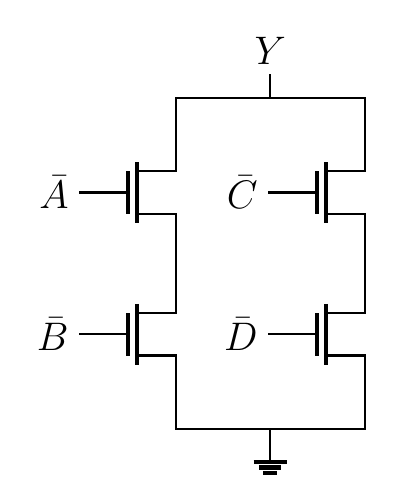
\begin{tikzpicture}[thick,font=\Large]\draw(0,0)--(-1.2,0)--(-1.2,-0.3);\node[nmos](m1)at(-1.2,-1.2){};\draw(-1.2,-0.3)--(m1.D)(m1.S)--(-1.2,-2.1);\draw(m1.G)--++(-.25,0)node[left]{$\bar A$};\node[nmos](m2)at(-1.2,-3.0){};\draw(-1.2,-2.1)--(m2.D)(m2.S)--(-1.2,-3.9000000000000004);\draw(m2.G)--++(-.25,0)node[left]{$\bar B$};\draw(-1.2,-3.9)--(-1.2,-4.2)--(0,-4.2);\draw(0,0)--(1.2,0)--(1.2,-0.3);\node[nmos](m3)at(1.2,-1.2){};\draw(1.2,-0.3)--(m3.D)(m3.S)--(1.2,-2.1);\draw(m3.G)--++(-.25,0)node[left]{$\bar C$};\node[nmos](m4)at(1.2,-3.0){};\draw(1.2,-2.1)--(m4.D)(m4.S)--(1.2,-3.9000000000000004);\draw(m4.G)--++(-.25,0)node[left]{$\bar D$};\draw(1.2,-3.9)--(1.2,-4.2)--(0,-4.2);\draw(0,0)--++(0,.3)node[above]{$Y$};\draw(0,-4.2)node[ground]{};\end{tikzpicture}
\end{document}
